% Author: Izaak Neutelings (July, 2017)
% based on code from a friend
\documentclass[border=1pt,tikz]{standalone}

\usepackage{amsmath} % for \dfrac
\usepackage{tikz}
\usepackage{calc} % for simple arithmetic
\tikzset{>=latex} % for LaTeX arrow head

\begin{document}





% TIMELINE - simple
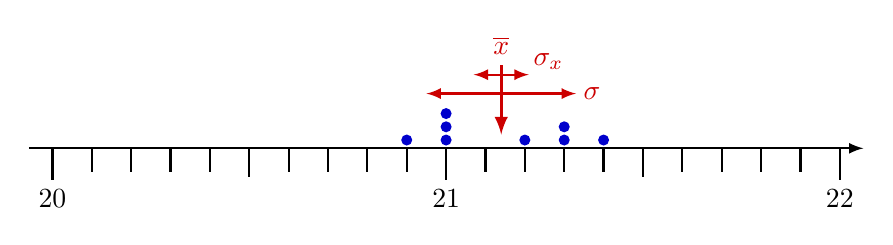
\begin{tikzpicture}[]
  \newcount\tZero; \tZero=20
  \def\w{10}    % width of axes
  \def\n{2}     % number of decades
  \def\lt{0.40} %  ten tick length
  \def\lf{0.36} % five tick length
  \def\lo{0.30} %  one tick length
  \def\r{0.07} %  dot radius
  
  %\def\tArrow#1#2{
  %  \def\tx{{(#1-\tZero)*\w/\n}};
  %  \draw[<-,thick,blue!80!black,align=center] (\tx,0*\lt) --++ (90+#2:0.8*\lt);
  %}
  \def\mydot(#1,#2){
    \def\tx{{(#1-\tZero)*\w/\n}};
    \fill[blue!80!black] (\tx,1.5*\r+#2*2.4*\r) circle (\r);
  }
  
  % AXIS
  %\draw[thick] (0,0) -- (\w,0);
  \draw[->,thick] (-\w*0.03,0) -- (\w*1.03,0);
  
  % TICKS
  \foreach \tick in {0,1,...,\n}{
    \def\x{{\tick*\w/\n}}
    \def\t{\the\numexpr \tZero+\tick \relax}
  	\draw[thick] (\x,0) --++ (0,-\lt) % ten tick
	             node[below] {\t};
	\ifnum \tick<\n
	  \draw[thick] ({(\x+\w/\n/2)},0) -- ({(\x+\w/\n/2)},-\lf); % five tick
      \foreach \ticko in {1,2,3,4,6,7,8,9}{
        \def\xo{{(\x+\ticko*\w/\n/10)}}
  	    \draw[thick] (\xo,0) --++ (0,-\lo);  % one tick
	}\fi
  }
  
  % LABEL
  \mydot(21.0,0)
  \mydot(21.0,1)
  \mydot(21.0,2)
  \mydot(21.2,0)
  \mydot(21.3,0)
  \mydot(21.3,1)
  \mydot(21.4,0)
  \mydot(20.9,0)
  
  \draw[<-,very thick,red!80!black]
    ({(21.14-\tZero)*\w/\n},2.5*\r) --++ (0,2.2*\lt)
    coordinate (A) node[above] {$\overline{x}$};
  \draw[<->,thick,red!80!black]
    (A)++(-0.19*\w/\n,-0.9*\lt) --++ (0.38*\w/\n,0)
    node[right=-1] {$\sigma$};
  \draw[<->,thick,red!80!black]
    (A)++(-0.07*\w/\n,-0.3*\lt) --++ (0.14*\w/\n,0)
    node[above right=-2] {$\sigma_x$};
  
\end{tikzpicture}



  
  

\end{document}
